%%\paragraph{}
MC based uncertainties are propagated in the analysis using standard CP group recommendations. These uncertainties can change both the shape and normalization of the signal and of the MC-based background prediction (Z+jets). The multijet and $t\bar{t}$ backgrounds normalisations are estimated with a data driven method (the likelihood fit). Since the shape for the $t\bar{t}$ component is taken from MC, the fit is redone for each MC variations.

\paragraph{Luminosity uncertainty}: The uncertainty on the combined 2015+2016 integrated luminosity is 2.1\%, assuming uncorrelated uncertainties between years. It is derived, following a methodology similar to that detailed in Refs. \cite{Aad:2013ucp} and \cite{ATLASlumi8TeV}, from a preliminary calibration of the luminosity scale using x-y beam-separation scans performed in August 2015 and May 2016. This uncertainty is applicable to the backgrounds with normalizations determined from simulation, and further propagated to the multijet prediction through data-driven background estimation procedure. It is expected to have a small impact on this analysis. This uncertainty is also applied to the signal normalization prediction

\paragraph{Large-R jet resolution and scale uncertainties}:
 The uncertainties on the jet energy and mass  (JES, JMS scale) are evaluated by the combined performance groups using track-to-calorimeter double ratios between data and MC, measured in dijet data~\cite{Aad:2013gja,BosonTagPreRec} . Discrepancies observed between data and MC are assigned as uncertainties on the energy/mass scales of the jet. Different correlation scenarios are supported by the Jet Substructure group, where all uncertainties can be decorrelated, fully correlated, or only correlated between energy and mass. Currently the latter is being used, know as the ``medium'' configuration.
The uncertainties on the jet energy, mass resolutions are estimated by applying a Gaussian smearing which degrades the nominal resolution by an absolute 2\% for $p_{T}$, relative 20\% for mass.
% Standard uncertainties on JES/JMS provided by jet substructure performance group.  JES
% determined in gamma+jet events, and JMS derived using calo/track jet ratios.  The JES_UP/JMR uncertainty is conservatively 20\% of the 
% intrinsic resolution in our signal sample.
%trimmed jets with $R=1.0$ are fully supported in the jet substructure performance group~\cite{JetSubst}.Systematic uncertainties for jet energy and mass scale (JES and JMS, respectively) are provided for supported \largeR jet collections by the JetUncertainties-00-09-63 tool as part of the standard Jet/MET uncertainty provider package~\cite{JESuncert}.  We use the $H \to b\bar{b}$ configurations:
%(\texttt{UJ2016\_CombinedMass\_strong.config}) 

%which includes uncertainties handling the heavy flavor differences between QCD (where the uncertainties are derived) and the signal $H$ jets.
%\Figref{jetsubstructure-uncert} shows the JES and JMS uncertainties provided for \antikt\ trimmed jets used in this analysis.
The uncertainties in our kinematic regime for signal yield predictions are below 7\% for JES/JMS. For $t\bar{t}$ yield predictions the uncertainties are $\sim$7-24\% for JES/JMS. Details are listed in section \ref{sec:boosted-systematics-numbers}. The uncertainties in our kinematic regime for signal yield predictions are below 7\% / 15\% for JER/JMR. For $t\bar{t}$ yield predictions the uncertainties are $\sim$4-27\% for JER/JMR. Details are listed in section \ref{sec:boosted-systematics-numbers}.

%The jet energy scale uncertainty 
%is derived with the $\gamma$-jet balance method for $pT < 800$~GeV and $|\eta| < $2.2, 
%and the track jets double ratio method for $pT > 800$~GeV and $|\eta| <$ 1.2. 
%The track jet double ratio method is used for the derivation of JMS uncertainties, in bins of $M/\pt$.
%Mass scale uncertainties are derived using 
%the track jets double ratio only, in the full \pt\ range and for $|\eta| <$ 2.0. 
%More details are given in~\cite{UJU}. These uncertainties are applied to all simulation samples.

%%%\paragraph{}
%Systematic uncertainties for energy and mass resolution are currently not well constrained, see \href{https://twiki.cern.ch/twiki/bin/viewauth/AtlasProtected/JetUncertainties2016PrerecLargeR}{link}. MC-based studies in 2010 implied that variations of the order of 20\% were possible. For \largeR jets used in this analysis, this is also validated with boosted W bosons in 2012 data~\cite{boostedW}. For each signal mass point, we smear the mass resolution of the \largeR trimmed jets by a Gaussian such that the intrinsic resolution is increased by 20\%. For jet energy resolution, the momentum is smeared with an aboslute 2\% uncertainty. The nominal MC mass resolution ($\sigma_{M}$) for every signal mass point is determined by fitting the reco\_M/truth\_M or distribution with a Gaussian, respectively. The reco\_M/truth\_M is found before the final $X_{hh}$ cut. Here, a truth trimmed jet is matched to the reconstructed trimmed jet within $dR<0.7$.

%%%\paragraph{}
%In all cases, the intrinsic resolution is small, due to the fact that each \largeR jet already has a more stable substructure after the two ghost-associated track jets requirement (it has been shown in the Jet Substructure group that \largeR jets with 2 or 3 subjets have a much better resolution than 
%\largeR jets with only one subjet).  The JMR is slightly larger than the JER for all mass points, and also slightly increases as a function of mass point while the JER slightly decreases as a function of mass point. To apply a 20\% systematic on the resolution, the jet mass is then smeared with a Gaussian with width 0.66*$\sigma_{M,\pt}$ (see~\cite{JetSubst}), also independently for every signal mass point.
%Figures \ref{fig:JERsyst_1} and \ref{fig:JERsyst_2} show the effect of the JER smearing for $c=1.0$ and $c=2.0$, respectively,
%on the leading and subleading \largeR jet \pt\ before any \pt\ cuts, as well as on the dijet mass after full selection. 



%%%\paragraph{}
%This smearing tends to increase the width of the dijet mass distributions, but with very little impact. The uncertainties in our kinematic regime for total signal yield predictions are $\sim 1 \%$ for JER, and between $\sim$1-2\% for JMR.  For $t\bar{t}$ yield predictions the uncertainties are $\sim$1-13\% for JER, and between $\sim$2-28\% for JMR. Details are listed in section \ref{sec:boosted-systematics-numbers}. \textbf{UPDATE}.

%We should note that the JMR uncertainty on $t\bar{t}$ is larger in the $4b$ SR than the $3b$ SR, even though the same $3b$ shape is used in both signal regions.  This is partially driven by the smaller statistics in the $4b$ region used in the background fit to constrain the background normalizations (which is done independently for the $3b$ and $4b$ SR's).

\paragraph{B-tagged track jet scale factor uncertainties}
\label{sec:b-tagging-unc}

The uncertainties related to the $b$-tagging efficiency calibrations as measured in $t\bar{t}$ events for track-jets are considered, using the official prescriptions. The procedure to define these calibrations is similar to that described in reference~\cite{Aad:2015ydr}.

The effect of the different experimental uncertainties on the signal yield is shown in section \ref{sec:boosted-systematics-numbers}. The signal yield uncertainty due to $b$-tagging is less than 30\% for the signal, and less than 12\% for the $t\bar{t}$ background yield. The main difference with respect to the previous result is on the $b$-tagging uncertainties, which have been reduced by approximately 50\%.
The total effect of the $b$-tagging uncertainty on the expected limits is shown in Sec.\,\ref{sec:statistical-analysis}, along with other uncertainties.

%%%\paragraph{}
%Calibrations, or correction factors in the form of scale factors per $p_{T}$ bin, for the $b$-tagging efficiency of $R=0.2$ track jets passing an MV2c10 weight cut corresponding to 77\% efficiency have been derived in \cite{ATL-COM-PHYS-2015-009,ATL-COM-PHYS-2015-1323}.  These calibrations are applied to the RS graviton signal samples, \ttbar\ and to the $Z$+jets simulation.  The calibrations also include uncertainties which modify the $b$-tagging efficiency and thus modify the signal (\ttbar\ and $Z$+jets) acceptance, and thus these uncertainties must be  propagated through the analysis. 
%
%%%\paragraph{}
%These calibrations are derived from Run 2 data for $b$-jets. In addition, the charm and light jet calibrations are taken from calo-jets, with an appropriate jet $p_{T}$ rescaling to account for the difference in calo and track jet $p_{T}$. Additional uncertainties are added to the charm and light calibrations to account for possible differences in track and calo jet calibrations.  More information can be found in \cite{ATL-PHYS-PUB-2015-035}.
%
%%%\paragraph{}
%The largest contributions to the systematic uncertainty on the Run 2 $b$-jet scale factors come predominantly from theoretical modeling, and from the uncertainties on the track reconstruction efficiency.  Specifically, \textbf{NUMBERS UPDATE}
%\begin{itemize}
%	\item The hadronization model, tested by comparing {\sc Powheg+Pythia} to {\sc Powheg+Herwig} $t\bar{t}$ samples, results in a 1-2\% uncertainty, depending on $p_{T}$ bin.
%	\item The choice of the Monte Carlo generator, tested by comparing {\sc Powheg+Herwig} to {\sc MC@NLO+Herwig} $t\bar{t}$ samples, results in a 1-6\% uncertainty, depending on $p_{T}$ bin.
%	\item The modeling of initial and final state radiation, tested by comparing two {\sc AcerMC+Pythia} $t\bar{t}$ samples with different tunes of the parameters to increase and decrease the amount of ISR /FSR, results in a 1-3\% uncertainty, depending on $p_{T}$ bin.
%	\item The modeling of the track reconstruction efficiency, tested by randomly throwing away tracks in track jets with a probability corresponding to the track reconstruction efficiency uncertainty, results in a 1-2\% uncertainty, depending on $p_{T}$ bin.
%\end{itemize}
%
%%%\paragraph{}
%Additional uncertainties, such as the muon and electron reconstruction efficiency, $p_{T}$ resolution,  and $p_{T}$ scale uncertainties, trigger efficiency, etc., have been included in the calibration but are seen to be sub-dominant. A full detailing of the systematics can be found in \cite{ATL-COM-PHYS-2015-009}.
%
%%%\paragraph{}
%In order to check for any additional uncertainties or mismodeling of the $b$-tagging performance in dense environments, where two $b$-jets are close by, a cross check of the $b$-tagging calibration has been performed in a boosted gluon$\to b\bar{b}$ jet sample as found in \cite{ATL-COM-PHYS-2014-1561}.  These studies show no major mismodeling of the Monte Carlo simulation inconsistent with the data within the $b$-tagging uncertainties. 
%
%%%\paragraph{}
%For track jets with $p_{T}>250$ GeV, not enough statistics are available in the data based analysis to provide an accurate calibration. As a result, an extrapolation is required. The extrapolation is performed only on the calibration uncertainty. The baseline scale factor for track jets with $p_{T}>250$ is taken to be the same as the 100-250 GeV bin, as is the baseline uncertainty. The extrapolation aims to include additional uncertainties that may affect the calibration uncertainties in the high $p_{T}$ bins that can not be calibrated directly from data. The extrapolation is performed in Monte Carlo, and relies on varying the inputs to $b$-tagging and examining the $b$-tagging efficiency under all of these variations. The variations include tracking efficiency, tracking resolution, and variations in the number fake and shared tracks. The variations observed with respect to the 100-250 GeV track jet $p_{T}$ bin are taken as the extrapolation uncertainty of the variation. The uncertainty from all variations are added in quadrature to estimate the full extrapolation uncertainty. \textbf{UPDATE}
%
%
%%%\paragraph{}
%The $b$-tagging calibrations are applied to the leading two track jets in each of the leading large-$R$ jets in each event.  In order to properly handle the correlations of the $b$-tagging calibration uncertainty between jets in an event, and between events, the $b$-tagging uncertainties are applied using the eigenvector approach, which computes the total covariance matrix including correlations of all $p_{T}$ bins in the calibration and decomposes them into a smaller number of eigenvector variations. The total effect of the $b$-tagging uncertainty on the expected limits is shown in Sec.\,\ref{sec:statistical-analysis}, along with other uncertainties.
%
%%%\paragraph{}
%The impact of the $b$-tagging uncertainties is 2-50\% on the $t\bar{t}$ background yield estimates.  The variation is larger for the signal samples, due to the large $b$-tag uncertainties for high-$p_T$ jets which are more common in the high mass samples.  As a result, the uncertainties on the signal yield vary between 15-60\% in the sensitive regions, depending on signal region ($3b$ or $4b$ or $2b$) and signal mass.
%
%%%\paragraph{}
%In particular, we notice a significant reduction of b-tagging systematic uncertainty in 3b signal region compared to 4b signal region. The reduced $b$-tagging uncertainty is due to the requirement that there must be one anti-tagged jet. For the signal, this is likely an anti-tagged $b$-jet. The uncertainty reduction occurs since when a $b$-tagged jet is calibrated with a scale factor $w_{sf}$ with uncertainties $\Delta w_{sf}$, any change in tagging efficiency must be corrected in the opposite direction for the anti-tagged jets in order to ensure that the total number of tagged plus anti-tagged jets does not change once the calibration is applied. Thus the anti-tagging calibration scale factor would be $w_{sf}^{anti} = (1 - w_{sf} \epsilon_{b}) / (1 - \epsilon_{b}) $ where $\epsilon_{b}$ is the tagging efficiency. From this equation, it is clear that a shift in the scale factor for tagged jets causes an anti-correlated shift in the anti-tagging efficiency scale factor. This anti-correlation in turn reduces the overall impact of the b-tagging uncertainty on the $3b$ SR. However, this anti-tagging efficiency scale factor is so large, that in $2bs$ SR, the total uncertainty will be dominated by the square of this factor, and hence it could be larger than $4b$'s $b$-tagging uncertainty.

%More details on this can be found in Appendix~\ref{app:boostedbtagsyst}.



\paragraph{\ttbar MC Uncertainty}
\label{sec:b-tagging-unc}
\hspace{0.1mm}\newline

%%\paragraph{}
In addition to the \ttbar fit uncertainties, following the recommendations, extra \ttbar MC samples are used with different varations: Hadronization, Fragmentation, Matrix Element and Additional Radiation. The top quark mass varations are also considered. The MC samples used are:

\noindent
\\
{\scriptsize
\verb|mc15_13TeV.410001.PowhegPythiaEvtGen_P2012radHi_ttbar_hdamp345_down_nonallhad.merge.DAOD_EXOT8.e3783_s2608_r7725_r7676_p2949|\\
\verb|mc15_13TeV.410002.PowhegPythiaEvtGen_P2012radLo_ttbar_hdamp172_up_nonallhad.merge.DAOD_EXOT8.e3783_s2608_r7725_r7676_p2949|\\
\verb|mc15_13TeV.410003.aMcAtNloHerwigppEvtGen_ttbar_nonallhad.merge.DAOD_EXOT8.e4441_s2726_r7772_r7676_p2949|\\
\verb|mc15_13TeV.410004.PowhegHerwigppEvtGen_UEEE5_ttbar_hdamp172p5_nonallhad.merge.DAOD_EXOT8.e3836_a766_a821_r7676_p2949|\\
\verb|mc15_13TeV.410008.aMcAtNloHerwigppEvtGen_ttbar_allhad.merge.DAOD_EXOT8.e3964_s2726_r7772_r7676_p2949|\\
\verb|mc15_13TeV.410022.Sherpa_CT10_ttbar_SingleLeptonP_MEPS_NLO.merge.DAOD_EXOT8.e3957_s2608_s2183_r7725_r7676_p2949|\\
\verb|mc15_13TeV.410022.Sherpa_CT10_ttbar_SingleLeptonP_MEPS_NLO.merge.DAOD_EXOT8.e3959_a766_a818_r7676_p2949|\\
\verb|mc15_13TeV.410023.Sherpa_CT10_ttbar_SingleLeptonM_MEPS_NLO.merge.DAOD_EXOT8.e3957_s2608_s2183_r7725_r7676_p2949|\\
\verb|mc15_13TeV.410023.Sherpa_CT10_ttbar_SingleLeptonM_MEPS_NLO.merge.DAOD_EXOT8.e3959_a766_a818_r7676_p2949|\\
\verb|mc15_13TeV.410024.Sherpa_CT10_ttbar_AllHadron_MEPS_NLO.merge.DAOD_EXOT8.e3957_s2608_s2183_r7725_r7676_p2949|\\
\verb|mc15_13TeV.410024.Sherpa_CT10_ttbar_AllHadron_MEPS_NLO.merge.DAOD_EXOT8.e3959_a766_a818_r7676_p2949|\\
\verb|mc15_13TeV.410037.PowhegPythiaEvtGen_P2012_ttbar_hdamp170_nonallhad.merge.DAOD_EXOT8.e4529_s2608_s2183_r7725_r7676_p2949|\\
\verb|mc15_13TeV.410038.PowhegPythiaEvtGen_P2012_ttbar_hdamp171p5_nonallhad.merge.DAOD_EXOT8.e4529_s2608_s2183_r7725_r7676_p2949|\\
\verb|mc15_13TeV.410039.PowhegPythiaEvtGen_P2012_ttbar_hdamp173p5_nonallhad.merge.DAOD_EXOT8.e4529_s2608_s2183_r7725_r7676_p2949|\\
\verb|mc15_13TeV.410040.PowhegPythiaEvtGen_P2012_ttbar_hdamp175_nonallhad.merge.DAOD_EXOT8.e4529_s2608_s2183_r7725_r7676_p2949|\\
\verb|mc15_13TeV.410041.PowhegPythiaEvtGen_P2012_ttbar_hdamp177p5_nonallhad.merge.DAOD_EXOT8.e4529_s2608_s2183_r7725_r7676_p2949|\\
\verb|mc15_13TeV.410042.PowhegPythiaEvtGen_P2012_ttbar_hdamp170_allhad.merge.DAOD_EXOT8.e4510_s2608_s2183_r7725_r7676_p2949|\\
\verb|mc15_13TeV.410043.PowhegPythiaEvtGen_P2012_ttbar_hdamp171p5_allhad.merge.DAOD_EXOT8.e4510_s2608_s2183_r7725_r7676_p2949|\\
\verb|mc15_13TeV.410044.PowhegPythiaEvtGen_P2012_ttbar_hdamp173p5_allhad.merge.DAOD_EXOT8.e4510_s2608_s2183_r7725_r7676_p2949|\\
\verb|mc15_13TeV.410045.PowhegPythiaEvtGen_P2012_ttbar_hdamp175_allhad.merge.DAOD_EXOT8.e4510_s2608_s2183_r7725_r7676_p2949|\\
\verb|mc15_13TeV.410046.PowhegPythiaEvtGen_P2012_ttbar_hdamp177p5_allhad.merge.DAOD_EXOT8.e4510_s2608_s2183_r7725_r7676_p2949|\\
\verb|mc15_13TeV.410161.PowhegPythiaEvtGen_P2012radHi_ttbar_hdamp345_down_allhad.merge.DAOD_EXOT8.e4837_s2726_r7772_r7676_p2949|\\
\verb|mc15_13TeV.410162.PowhegPythiaEvtGen_P2012radLo_ttbar_hdamp172p5_up_allhad.merge.DAOD_EXOT8.e4837_s2726_r7772_r7676_p2949|\\
\verb|mc15_13TeV.410163.PowhegHerwigppEvtGen_UEEE5_ttbar_hdamp172p5_allhad.merge.DAOD_EXOT8.e4836_s2726_r7772_r7676_p2949|
}
\noindent

%%\paragraph{}
These \ttbar samples are used to replace the normal had and nonhad MCs, stiched with Mtt slices samples, and the variation in the \ttbar yield and background predictions are considered. The variation in total background, with different \ttbar MC sample as input is tested. This is shown in Figure ~\ref{fig:ttbar-MC}. Therefore, this uncertainty is considered limited by the MC statistics and dropped from the final list.

\begin{figure}[htbp!]
\begin{center} 
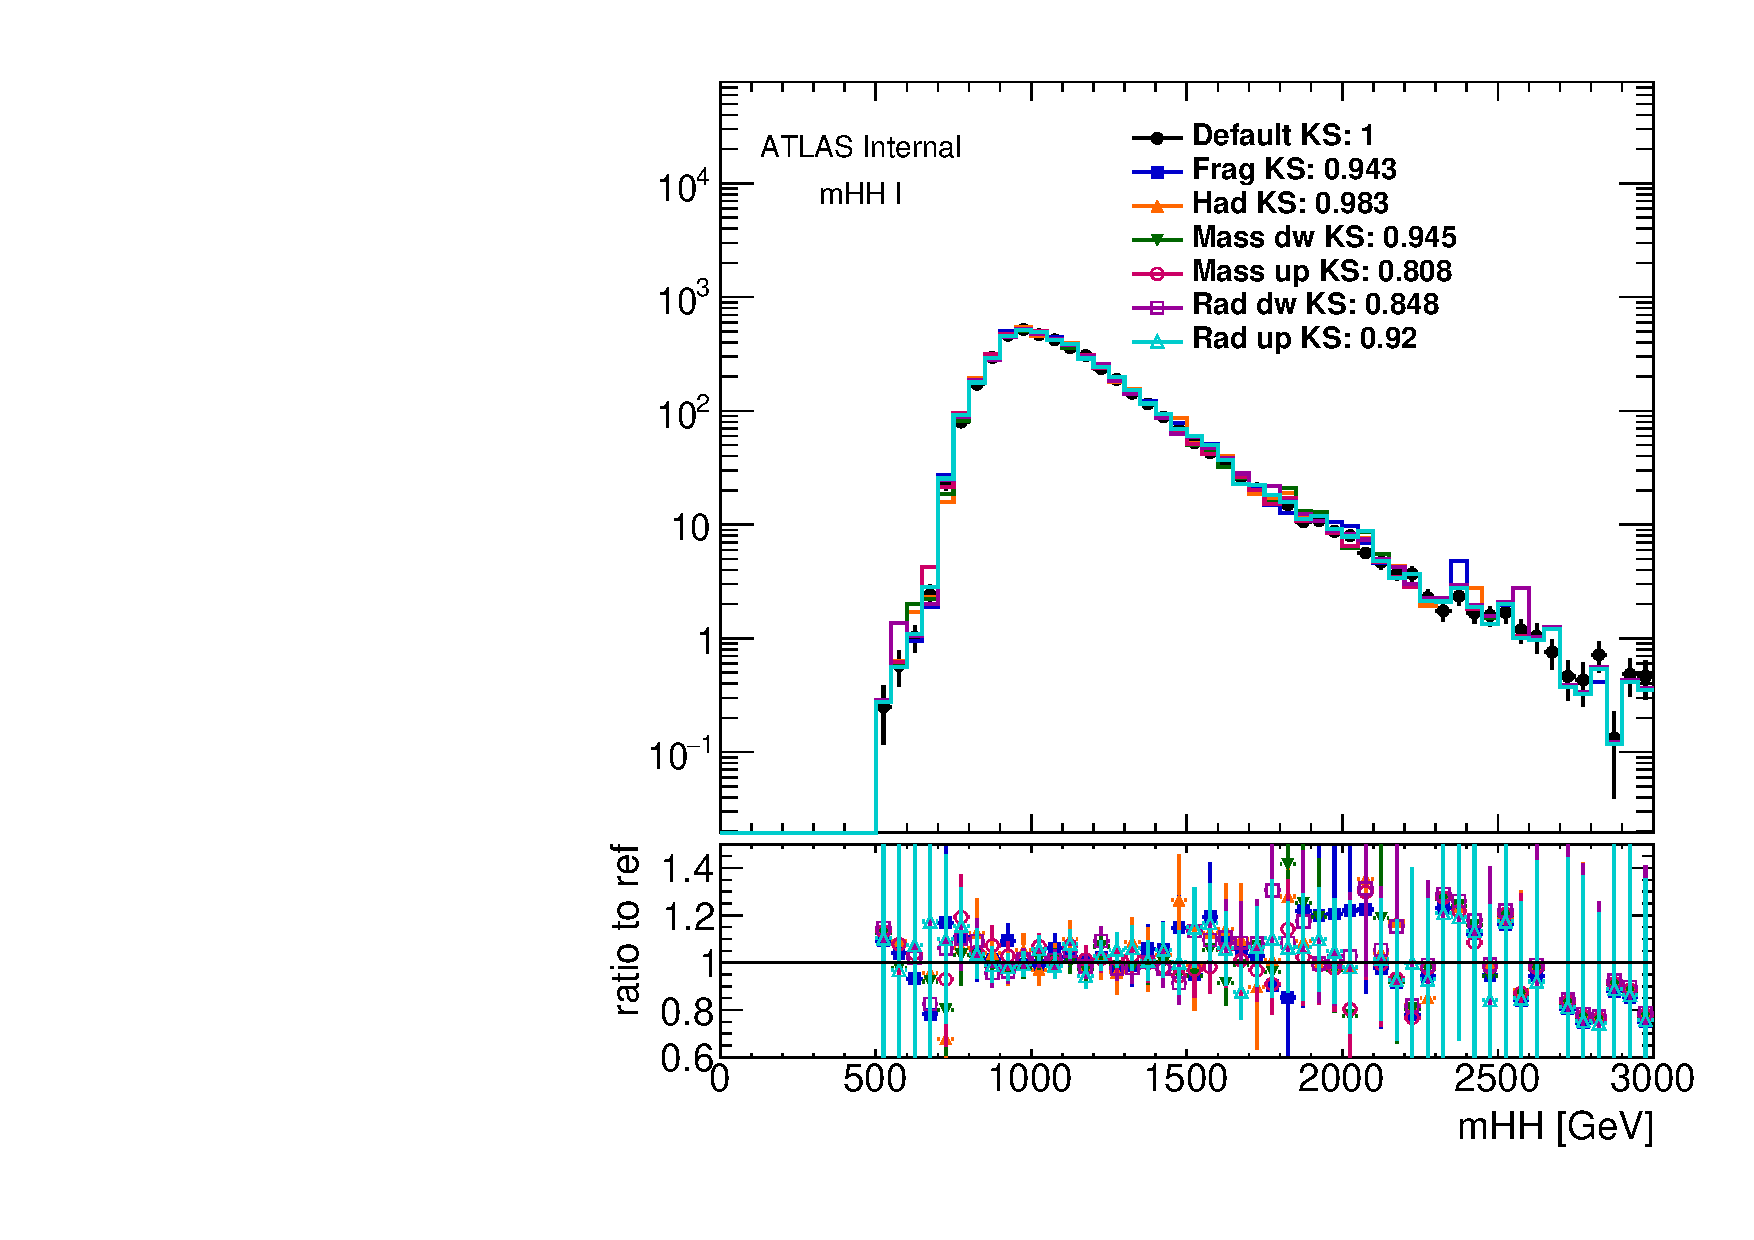
\includegraphics[width=0.48\textwidth,angle=-90]{figures/boosted/Other/directcompare_mHH_l_1_TwoTag_split_Top_syst_stat_postfit_all_.pdf}
\caption{Total background estimation (qcd + \ttbar) with different \ttbar MC variations. The different variations agree with the default within the statistical uncertainties.}
\label{fig:ttbar-MC}
\end{center}
\end{figure}
%The total varation on \ttbar yield in signal region is between 12-58\%. These are shown in section \ref{sec:boosted-systematics-numbers}. 
